\documentclass[tikz,border=10pt]{standalone}

\usepackage{xcolor}
\usetikzlibrary{arrows.meta,positioning}

\begin{document}

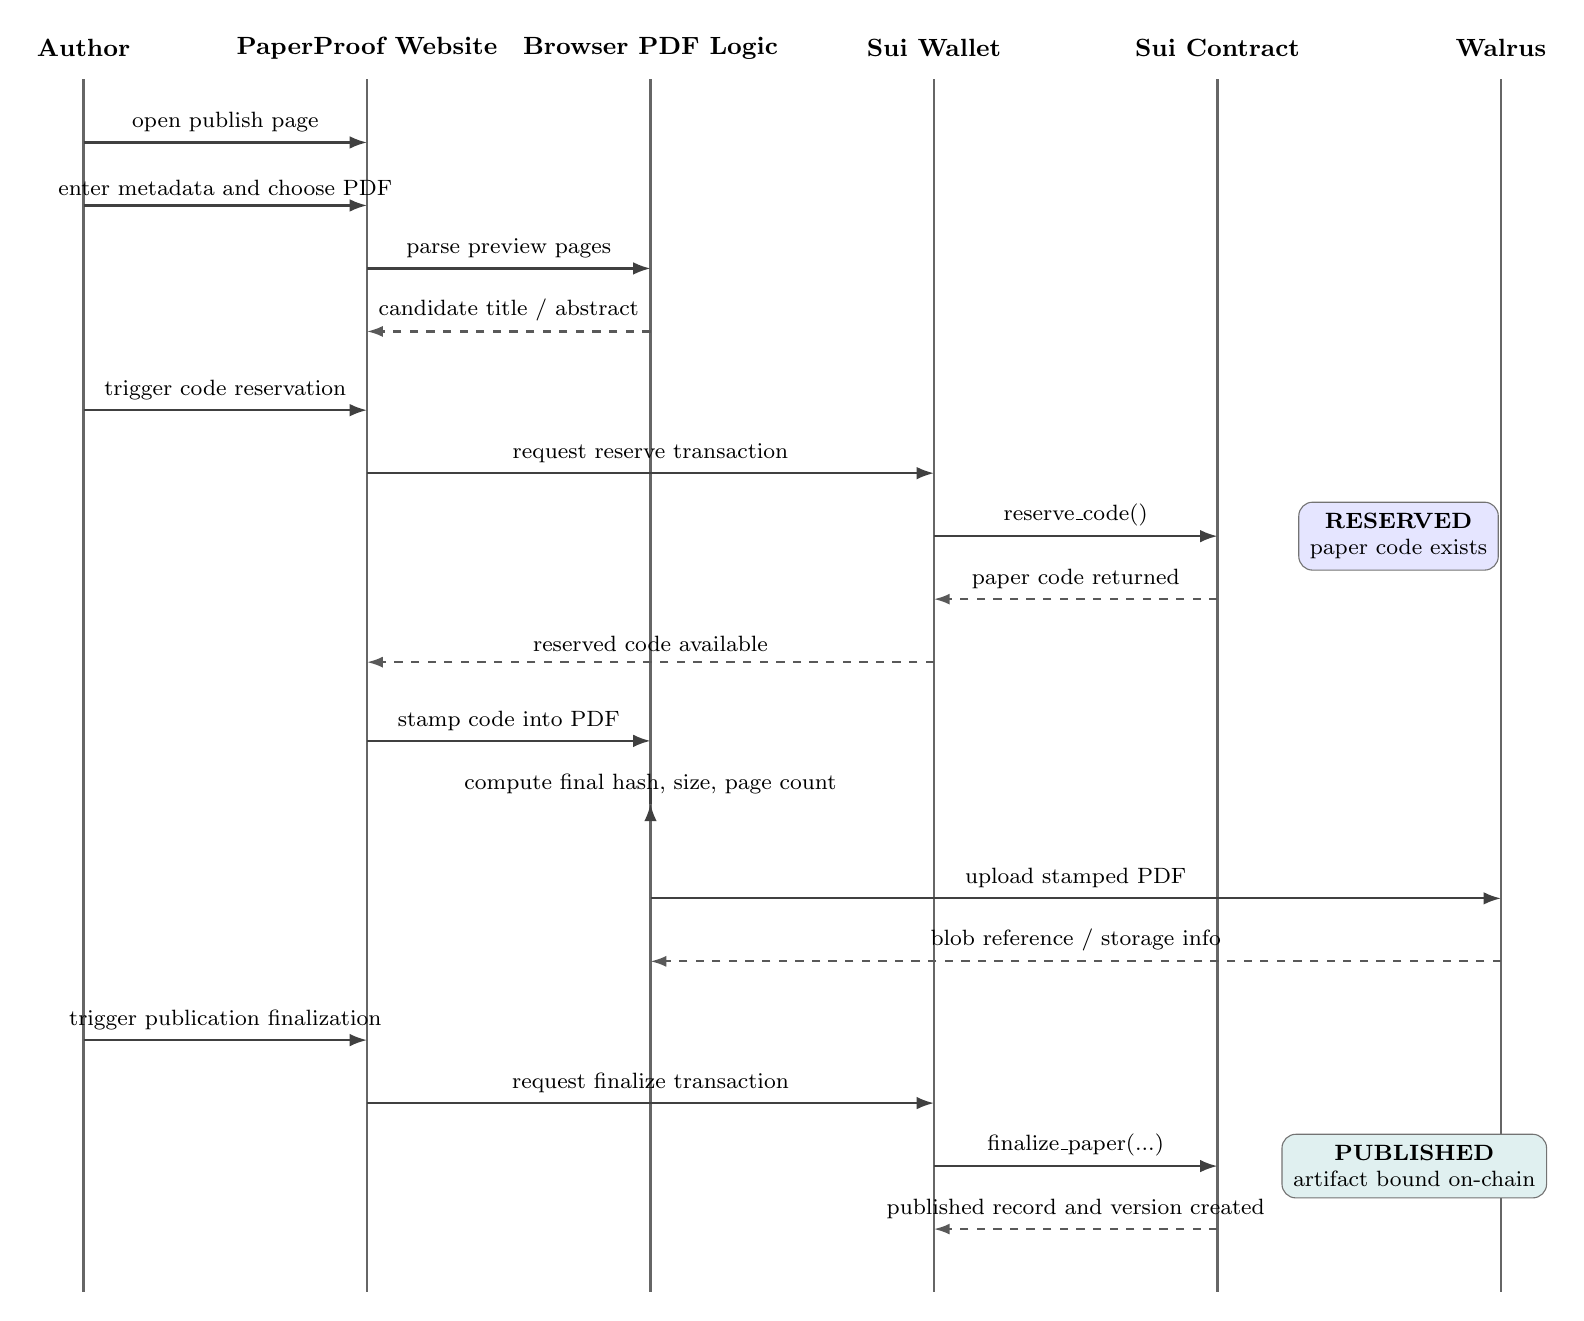
\begin{tikzpicture}[
    font=\small,
    lifeline/.style={draw=black!60, thick},
    msg/.style={-{Latex[length=2.2mm,width=1.6mm]}, thick, draw=black!75},
    reply/.style={-{Latex[length=2.0mm,width=1.4mm]}, thick, dashed, draw=black!65},
    note/.style={
        rectangle,
        rounded corners=4pt,
        draw=black!40,
        fill=gray!8,
        align=left,
        font=\footnotesize,
        inner sep=5pt
    },
    state/.style={
        rectangle,
        rounded corners=5pt,
        draw=black!55,
        fill=blue!10,
        align=center,
        font=\footnotesize,
        inner sep=4pt
    }
]

% =========================================================
% Participants
% =========================================================
\node at (0,0) {\textbf{Author}};
\node at (3.6,0) {\textbf{PaperProof Website}};
\node at (7.2,0) {\textbf{Browser PDF Logic}};
\node at (10.8,0) {\textbf{Sui Wallet}};
\node at (14.4,0) {\textbf{Sui Contract}};
\node at (18.0,0) {\textbf{Walrus}};

% Lifelines
\draw[lifeline] (0,-0.4) -- (0,-15.8);
\draw[lifeline] (3.6,-0.4) -- (3.6,-15.8);
\draw[lifeline] (7.2,-0.4) -- (7.2,-15.8);
\draw[lifeline] (10.8,-0.4) -- (10.8,-15.8);
\draw[lifeline] (14.4,-0.4) -- (14.4,-15.8);
\draw[lifeline] (18.0,-0.4) -- (18.0,-15.8);

% =========================================================
% Sequence messages
% =========================================================

% Step 1
\draw[msg] (0,-1.2) -- node[above, font=\footnotesize] {open publish page} (3.6,-1.2);
\draw[msg] (0,-2.0) -- node[above, font=\footnotesize] {enter metadata and choose PDF} (3.6,-2.0);
\draw[msg] (3.6,-2.8) -- node[above, font=\footnotesize] {parse preview pages} (7.2,-2.8);
\draw[reply] (7.2,-3.6) -- node[above, font=\footnotesize] {candidate title / abstract} (3.6,-3.6);

% Step 2 reserve
\draw[msg] (0,-4.6) -- node[above, font=\footnotesize] {trigger code reservation} (3.6,-4.6);
\draw[msg] (3.6,-5.4) -- node[above, font=\footnotesize] {request reserve transaction} (10.8,-5.4);
\draw[msg] (10.8,-6.2) -- node[above, font=\footnotesize] {reserve\_code()} (14.4,-6.2);
\draw[reply] (14.4,-7.0) -- node[above, font=\footnotesize] {paper code returned} (10.8,-7.0);
\draw[reply] (10.8,-7.8) -- node[above, font=\footnotesize] {reserved code available} (3.6,-7.8);

\node[state] at (16.7,-6.2) {\textbf{RESERVED}\\paper code exists};

% Step 3 / 4
\draw[msg] (3.6,-8.8) -- node[above, font=\footnotesize] {stamp code into PDF} (7.2,-8.8);
\draw[msg] (7.2,-9.6) -- node[above, font=\footnotesize] {compute final hash, size, page count} (7.2,-9.6);

% Step 5
\draw[msg] (7.2,-10.8) -- node[above, font=\footnotesize] {upload stamped PDF} (18.0,-10.8);
\draw[reply] (18.0,-11.6) -- node[above, font=\footnotesize] {blob reference / storage info} (7.2,-11.6);

% Step 6 finalize
\draw[msg] (0,-12.6) -- node[above, font=\footnotesize] {trigger publication finalization} (3.6,-12.6);
\draw[msg] (3.6,-13.4) -- node[above, font=\footnotesize] {request finalize transaction} (10.8,-13.4);
\draw[msg] (10.8,-14.2) -- node[above, font=\footnotesize] {finalize\_paper(...)} (14.4,-14.2);
\draw[reply] (14.4,-15.0) -- node[above, font=\footnotesize] {published record and version created} (10.8,-15.0);

\node[state, fill=teal!12] at (16.9,-14.2) {\textbf{PUBLISHED}\\artifact bound on-chain};

\end{tikzpicture}

\end{document}
